\chapter{Data Source and Representation}
The dataset used as a resource to populate the database solutions is called EMAP; a freely available anatomical ontology of the developmental stages of mouse embryos. The EMAP dataset was chosen for this project as my supervisor has much experience in the field and would be able to assist me with any queries I had regarding the data. The size and granularity of the EMAP dataset also meets the criteria which will be required to test the database solutions (Section REQUIREMENTS), explore the limitations of each database comparatively and pose insight into the overall performance of each database.

\section{EMAP}
The \textit{Edinburgh Mouse Atlas Project} (EMAP) is an ongoing research project to develop a digital atlas of mouse development. The objective of the EMAP is to implement a digital model of mouse embryos for each time stage in development (EMAP Ref). The collated model embryo data is then used to form a database from which further research can be conducted and experiments can be mapped.
 
Each time step in the digital model are named \textit{Theiler Stages} inspired by the research conducted by Karl Theiler (REF). A Theiler Stage defines the development of a mouse embryo by the form and structure of organisms and their specific structural features. (Theiler Ref) There are 26 individual Theiler Stages which define the growth and evolution of the mouse embryo. The Theiler Stage scheme comprises of both the anatomical developmental stage definition and the estimated length of time since conception. Each Theiler Stage also provides a brief description of the anatomy and any significant changes between the current and previous stage.

Theiler proposed using this scheme as embryos at the same developmental age can have evolved at different rates and therefore exhibit different structural characteristics. (REF Theiler 1989) The EMAP has developed a collection of three dimensional computer models which illustrate and summarise each Theiler Stage. (EMAP website link). 

The anatomy generated at each Theiler Stage has an associated ontological representation. Each provides an alternative aspect of the evolution of a mouse embryo which corresponds with a respective Theiler Stage. The abbreviated term EMAP carries a certain amount of ambiguity as it is refers to the name of the project, and one of the stages in the implemented anatomy. (Ref Ken thesis)  For the purpose of this project the main anatomy to be utilised is the aggregated non stage specific Edinburgh Mouse Atlas Project Abstract (EMAPA) anatomy. The reasoning behind this and comparative ontological anatomies such as EMAP and Edinburgh Mouse Atlas of Gene Expression (EMAGE) are discussed below.

\subsection{EMAP anatomy}
The EMAP anatomy ontology was originally developed to deliver a stage-specific anatomical structure for the developing laboratory mouse. As the EMAP research has progressed, the ontology has followed suit, and is continually under development.

The original EMAP anatomy ontology consists of a series of relational components organised in a hierarchical tree structure which utilise "part-of" relations and subdivisions which encompass each Theiler Stage.(EMAP REF) The intention behind the implementation of the original ontology structure was to "...describe the whole embryo as a tree of anatomical structures successively divided into non-overlapping named parts". (EMAP REF)

Each of the Theiler Stage components has an appropriately named term label, known as the \textit{short name} which describes each respective component. Each Theiler Stage also has a \textit{full name} which comes in the form of the components entire hierarchical path (EMAP REF). Neither the \textit{full} nor \textit{short} anatomical name of each component are required to be distinct and can appear in several Theiler Stages. Therefore to avoid ambiguity each component can be addressed by a unique identifier. The unique identifier is in the form of the relevant anatomy followed by a number (EMAP:number). For example "choroid plexus" is the short name of TS20/mouse/body region/head/brain/choroid plexus and has a has unique identifier of EMAP:4218.

The EMAP hierarchical structure facilitates the need for basic "data annotation and integration" however a combination of the lack of hierarchical views, missing or poorly represented Theiler Stages and label name ambiguity exposed the limitations of the EMAP structure. As a result the need for a hybrid "abstract" version of the anatomy was identified and subsequently developed; EMAPA. (EMAP REF) Thus the EMAPA anatomy will be the main data source for this work.

The research surrounding the EMAP resource is continually being developed, thus the growth of the project as a whole is progressively increasing with the richness of data at the heart (EMAP REF). The EMAPA ontology discussed below (Section \ref{emapaanatomy} is now considered the primary data source thus the EMAP dataset is only available in a combined EMAP and EMAPA standard ontological format developed by the Open Biological Ontologies (OBO) consortium (Section \ref{obo}).


\subsection{EMAPA anatomy}\label{emapaanatomy}
The EMAPA is a refined and algorithmically developed non-stage specific anatomical ontology \textit{abstract} representation of the EMAP anatomy. The EMAPA implementation replaces the EMAP hierarchical tree structure for a \textit{directed acyclic graph} structure; a graph in which it is impossible to start at some vertex v and follow a sequence of edges that eventually loops back to v again.(GRAPH REF) Thus enabling the ability to represent multiple parental relationships and other forms of "is-a" relations where appropriate. (EMAP REF)

Each anatomical component in the EMAPA anatomy is identified as a single term, coupled with the appropriate start and end Theiler Stage at which the component is considered to be present in the developing embryo. (EMAP REF) With the aim of enhancing user experience, the EMAPA anatomy  implements an alternative naming convention from the EMAP anatomy replacing full path names for components to \textit{"print names"}\begin{center}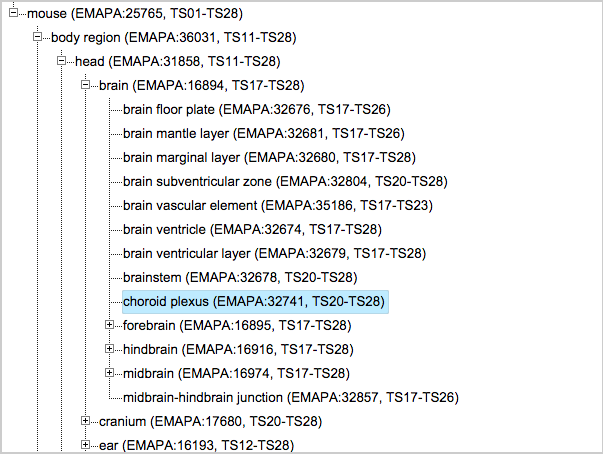
\includegraphics[width=1\linewidth]{images/emapachoroidplexus}\end{center}. Using the above example for comparison, "EMAP:4218" in the EMAP anatomy becomes "TS20 brain choroid plexus" in EMAPA. This naming convention supplements the requirement of uniqueness and is easily comprehensible. EMAPA 32741  

The EMAPA ontology is available in a standard ontological format developed by the Open Biological Ontologies (OBO) consortium (Section \ref{obo}) and is also available in a Web Ontology Language (OWL); a standard produced from W3C (Section \ref{owl}).This enhanced version of the ontology EMAPA, is now considered to be the primary EMAP anatomy ontology thus will be the main source for the work on this project.


\subsection{EMAGE anatomy}

\subsubsection{EMA Database}\label{emadb}



